\documentclass[11pt,a4paper]{article}

% French
\usepackage[utf8x]{inputenc}
\usepackage[frenchb]{babel}
\usepackage[T1]{fontenc}
\usepackage{lmodern}
\usepackage{ifthen}

% Color
% cfr http://en.wikibooks.org/wiki/LaTeX/Colors
\usepackage{color}
\usepackage[usenames,dvipsnames,svgnames,table]{xcolor}
\definecolor{dkgreen}{rgb}{0.25,0.7,0.35}
\definecolor{dkred}{rgb}{0.7,0,0}

% Floats and referencing
\newcommand{\sectionref}[1]{section~\ref{sec:#1}}
\newcommand{\annexeref}[1]{annexe~\ref{ann:#1}}
\newcommand{\figuref}[1]{figure~\ref{fig:#1}}
\newcommand{\tabref}[1]{table~\ref{tab:#1}}
\usepackage{xparse}
\NewDocumentEnvironment{myfig}{mm}
{\begin{figure}[!ht]\centering}
{\caption{#2}\label{fig:#1}\end{figure}}

% Listing
\usepackage{listings}
\lstset{
  numbers=left,
  numberstyle=\tiny\color{gray},
  basicstyle=\rm\small\ttfamily,
  keywordstyle=\bfseries\color{dkred},
  frame=single,
  commentstyle=\color{gray}=small,
  stringstyle=\color{dkgreen},
  %backgroundcolor=\color{gray!10},
  %tabsize=2,
  rulecolor=\color{black!30},
  %title=\lstname,
  breaklines=true,
  framextopmargin=2pt,
  framexbottommargin=2pt,
  extendedchars=true,
  inputencoding=utf8x
}

\newcommand{\matlab}{\textsc{Matlab}}
\newcommand{\octave}{\textsc{GNU/Octave}}
\newcommand{\qtoctave}{\textsc{QtOctave}}
\newcommand{\oz}{\textsc{Oz}}
\newcommand{\java}{\textsc{Java}}
\newcommand{\clang}{\textsc{C}}
\newcommand{\keyword}{mot clef}

% Math symbols
\usepackage{amsmath}
\usepackage{amssymb}
\usepackage{amsthm}
\DeclareMathOperator*{\argmin}{arg\,min}
\DeclareMathOperator*{\argmax}{arg\,max}

% Sets
\newcommand{\Z}{\mathbb{Z}}
\newcommand{\R}{\mathbb{R}}
\newcommand{\Rn}{\R^n}
\newcommand{\Rnn}{\R^{n \times n}}
\newcommand{\C}{\mathbb{C}}
\newcommand{\K}{\mathbb{K}}
\newcommand{\Kn}{\K^n}
\newcommand{\Knn}{\K^{n \times n}}

% Chemistry
\newcommand{\std}{\ensuremath{^{\circ}}}
\newcommand\ph{\ensuremath{\mathrm{pH}}}

% Theorem and definitions
\theoremstyle{definition}
\newtheorem{mydef}{Définition}
\newtheorem{mynota}[mydef]{Notation}
\newtheorem{myprop}[mydef]{Propriétés}
\newtheorem{myrem}[mydef]{Remarque}
\newtheorem{myform}[mydef]{Formules}
\newtheorem{mycorr}[mydef]{Corrolaire}
\newtheorem{mytheo}[mydef]{Théorème}
\newtheorem{mylem}[mydef]{Lemme}
\newtheorem{myexem}[mydef]{Exemple}
\newtheorem{myineg}[mydef]{Inégalité}

% Unit vectors
\usepackage{esint}
\usepackage{esvect}
\newcommand{\kmath}{k}
\newcommand{\xunit}{\hat{\imath}}
\newcommand{\yunit}{\hat{\jmath}}
\newcommand{\zunit}{\hat{\kmath}}

% rot & div & grad & lap
\DeclareMathOperator{\newdiv}{div}
\newcommand{\divn}[1]{\nabla \cdot #1}
\newcommand{\rotn}[1]{\nabla \times #1}
\newcommand{\grad}[1]{\nabla #1}
\newcommand{\gradn}[1]{\nabla #1}
\newcommand{\lap}[1]{\nabla^2 #1}


% Elec
\newcommand{\B}{\vec B}
\newcommand{\E}{\vec E}
\newcommand{\EMF}{\mathcal{E}}
\newcommand{\perm}{\varepsilon} % permittivity

\newcommand{\bigoh}{\mathcal{O}}
\newcommand\eqdef{\triangleq}

\DeclareMathOperator{\newdiff}{d} % use \dif instead
\newcommand{\dif}{\newdiff\!}
\newcommand{\fpart}[2]{\frac{\partial #1}{\partial #2}}
\newcommand{\ffpart}[2]{\frac{\partial^2 #1}{\partial #2^2}}
\newcommand{\fdpart}[3]{\frac{\partial^2 #1}{\partial #2\partial #3}}
\newcommand{\fdif}[2]{\frac{\dif #1}{\dif #2}}
\newcommand{\ffdif}[2]{\frac{\dif^2 #1}{\dif #2^2}}
\newcommand{\constant}{\ensuremath{\mathrm{cst}}}

% Numbers and units
\usepackage[squaren, Gray]{SIunits}
\usepackage{sistyle}
\usepackage[autolanguage]{numprint}
%\usepackage{numprint}
\newcommand\si[2]{\numprint[#2]{#1}}
\newcommand\np[1]{\numprint{#1}}

\newcommand\strong[1]{\textbf{#1}}
\newcommand{\annexe}{\part{Annexes}\appendix}

% Bibliography
\newcommand{\biblio}{\bibliographystyle{plain}\bibliography{biblio}}

\usepackage{fullpage}
% le `[e ]' rend le premier argument (#1) optionnel
% avec comme valeur par défaut `e `
\newcommand{\hypertitle}[7][e ]{
\usepackage{hyperref}
{\renewcommand{\and}{\unskip, }
\hypersetup{pdfauthor={#6},
            pdftitle={Synth\`ese d#1#2 Q#3 - L#4#5},
            pdfsubject={#2}}
}

\title{Synth\`ese d#1#2 Q#3 - L#4#5}
\author{#6}

\begin{document}

\ifthenelse{\isundefined{\skiptitlepage}}{
\begin{titlepage}
\maketitle

 \paragraph{Informations importantes}
   Ce document est grandement inspiré de l'excellent cours
   donné par #7 à l'EPL (École Polytechnique de Louvain),
   faculté de l'UCL (Université Catholique de Louvain).
   Il est écrit par les auteurs susnommés avec l'aide de tous
   les autres étudiants, la vôtre est donc la bienvenue.
   Il y a toujours moyen de l'améliorer, surtout si le cours
   change car la synthèse doit alors être modifiée en conséquence.
   On peut retrouver le code source à l'adresse suivante
   \begin{center}
     \url{https://github.com/Gp2mv3/Syntheses}.
   \end{center}
   On y trouve aussi le contenu du \texttt{README} qui contient de plus
   amples informations, vous êtes invité à le lire.

   Il y est indiqué que les questions, signalements d'erreurs,
   suggestions d'améliorations ou quelque discussion que ce soit
   relative au projet
   sont à spécifier de préférence à l'adresse suivante
   \begin{center}
     \url{https://github.com/Gp2mv3/Syntheses/issues}.
   \end{center}
   Ça permet à tout le monde de les voir, les commenter et agir
   en conséquence.
   Vous êtes d'ailleurs invité à participer aux discussions.

   Vous trouverez aussi des informations dans le wiki
   \begin{center}
     \url{https://github.com/Gp2mv3/Syntheses/wiki}.
   \end{center}
   comme le statut des synthèses pour chaque cours
   \begin{center}
     \url{https://github.com/Gp2mv3/Syntheses/wiki/Status}.
   \end{center}
   vous pouvez d'ailleurs remarquer qu'il en manque encore beaucoup,
   votre aide est la bienvenue.

   Pour contribuer au bug tracker et au wiki, il vous suffira de
   créer un compte sur Github.
   Pour interagir avec le code des synthèses,
   il vous faudra installer \LaTeX.
   Pour interagir directement avec le code sur Github,
   vous devez utiliser \texttt{git}.
   Si cela pose problème,
   nous sommes évidemment ouverts à des contributeurs envoyant leurs
   changements par mail ou n'importe quel autre moyen.
\end{titlepage}
}{}

\ifthenelse{\isundefined{\skiptableofcontents}}{
\tableofcontents
}{}
}



\usepackage[usenames,dvipsnames]{xcolor}
\usepackage{graphicx}
\usepackage{url} 
\usepackage[toc]{appendix}
\usepackage{array}
\usepackage[final]{pdfpages}
\usepackage{listings}
\usepackage[Lenny]{fncychap}
\usepackage{verbatim}
\usepackage[top=1.5cm, bottom=1.5cm, left=1.5cm, right=1.5cm]{geometry}
\usepackage[rightcaption]{sidecap}
\usepackage{color}
\usepackage{here}
\usepackage{caption}
\usepackage{subcaption}
\providecommand{\e}[1]{\ensuremath{\times 10^{#1}}}
\usepackage{adjustbox}
\definecolor{lightorange}{RGB}{255,247,170}

\newenvironment{orangebox}{%
    \noindent
    \adjustbox{innerenv={varwidth}[c]{0.9\linewidth},margin=\fboxsep+.25cm \fboxsep+.2cm,bgcolor=lightorange,frame,center}\bgroup
}{%
    \egroup
}
\definecolor{lightsteel}{RGB}{176,196,222}

\newenvironment{bluebox}{%
    \noindent
    \adjustbox{innerenv={varwidth}[c]{0.9\linewidth},margin=\fboxsep+.25cm \fboxsep+.2cm,bgcolor=lightsteel,frame,center}\bgroup
}{%
    \egroup
}

\usepackage{accents}
\makeatletter
\newcommand{\sbullet}{%
  \hbox{\fontfamily{lmr}\fontsize{.4\dimexpr(\f@size pt)}{0}\selectfont$\circ\circ$}}
\DeclareRobustCommand{\mecacc}{\accentset{\sbullet}}
\makeatother

\usepackage{tikz}

\hypertitle{Cinématique et dynamique des machines Mémo}{4}{MECA}{1953}{Maxime De Mol}{Maxime De Mol}

\boldmath
\section*{\centering \fbox{Cinématique et Dynamique des Machines}}
\vspace{11pt}
\subsection*{1. Rappels de cinématique}
Théorème d'Euler $\Rightarrow$ \\
“ Tout déplacement d’un solide ayant {\color{orange}un point} fixe est une {\color{orange}rotation} autour d’{\color{orange}un axe} [fixe] e passant par ce point ”\\
$\rightarrow$ 3 dl $\rightarrow$ 2 pour orienter l’axe e ($\alpha$, $\beta$) + 1 autour de l’axe ($\theta$)\\

Propriétés utiles pour Chasles:\\
$\bullet$ Rotations successives autour d’axes $a_i$ parallèles $\Leftrightarrow$ Rotation autour d’un axe a parallèle aux $a_i$\\
$\bullet$ Deux rotations successives (axes $\parallel$) d’angles $\alpha$ et $-\alpha$  $\Leftrightarrow$ Rotation autour d’un axe a rejeté à l’infini $\Rightarrow$ Translation !\\
$\Rightarrow$ Une translation peut (donc) être remplacée par un couple de rotations\\

Théorème de Chasles $\Rightarrow$ \\
“ Un déplacement fini {\color{orange}quelconque} d’un solide peut être représenté par la {\color{orange}combinaison} d’un {\color{orange}translation} et d’une {\color{orange}rotation} ”\\
$\Rightarrow$ Déplacement fini quelconque $\Rightarrow$ mouvement “ hélicoïdale ”\\

Déplacement infinitésimal = cas particulier d'un déplacement fini $\Rightarrow$ axe hélicoïdal instantané\\
Propriété supplémentaire : rotations infinitésimales commutatives\\
$A_3A_2A_1 = A_1A_2A_3 = A_1A_3A_2 = ...$\\

\begin{bluebox}
\begin{tabbing}
ttttttttttttttttttttttt\=tttttttttttttttttttttttttttttttttttttttttttttttttttttttttttttttttttttttttttt\kill
Pour rappel, les matrices de rotation: \\\\
\>$A^{(1)}(\theta)= \begin{pmatrix}
1&0&0 \\
0&\cos\theta&-\sin\theta\\
0&\sin\theta&\cos\theta
\end{pmatrix}$\\\\
\>$A^{(2)}(\theta)= \begin{pmatrix}
\cos\theta&0&-\sin\theta \\
0&1&0\\
\sin\theta&0&\cos\theta
\end{pmatrix}$\\\\
\>$A^{(3)}(\theta)= \begin{pmatrix}
\cos\theta&-\sin\theta&0\\
\sin\theta&\cos\theta&0\\
0&0&1\\
\end{pmatrix}$\\
\end{tabbing}
\end{bluebox}\\\\

\begin{orangebox}
Mouvement général d’un solide = \\
{\color{orange}Séquence} de mouvements {\color{orange}hélicoïdaux} autour d’{\color{orange}axes hélicoïdaux instantanés} successifs
\end{orangebox}\\\\

\begin{orangebox}
“ La {\color{orange}projection} des vitesses en deux points d’un solide sur la droite qui les relie est la\\ même ”
\end{orangebox}\\\\

\begin{bluebox}
\begin{tabbing}
tttttttttttttttttttttttt\=tttttttttttttttttttttttttttttttttttttttt\=ttttttt\=tttttttttttttttttttttttttttt\kill
Vitesse absolue d'un point M: \\
\>$\vec{v}_M = \vec{v}_p+\mathring{\vec{p}}_M+\vec{\omega}\times\vec{p}_M$ \> avec \>$\mathring{\vec{p}}_M = [\vec{x}_\alpha]^T\dot{p}_M$\\
\>\>\>$\vec{\omega} = [\vec{x}_\alpha]^T\omega$\\
\>\>\>$\tilde{\omega} = A\dot{A}^T$
\end{tabbing}
\end{bluebox}\\\\

\begin{bluebox}
\begin{tabbing}
tttttttttttttttttttttttttttttttttttttttttttttttttttttttttttttttttttttttttt\=ttttttt\=tttttttttttttttttt\kill
Accélération absolue d'un point M: \\
$\vec{a}_M = \vec{a}_p+\mathring{\vec{\omega}}\times\vec{p}_M+\vec{\omega}\times(\vec{\omega}\times\vec{p}_M)+\mecacc{\vec{p}}_M+2\vec{\omega}\times\mathring{\vec{p}}_M$ \> avec \>$\mecacc{\vec{p}}_M = [\vec{x}_\alpha]^T\ddot{p}_M$\\
\>\>$\dot{\vec{\omega}} = \mathring{\vec{\omega}}$\\
Accélération centripète: $\vec{\omega}\times(\vec{\omega}\times\vec{p}_M)$\\
Accélération de Coriolis: $2\vec{\omega}\times\mathring{\vec{p}}_M$
\end{tabbing}
\end{bluebox}\\\\

Axoïdes:\\
$\bullet$ {\color{orange}Axoïde fixe} = ensemble des droites de {\color{orange}l’espace} qui coïncident avec les axes hélicoïdaux successifs (= \underline{surface réglée fixe})\\
$\bullet$ {\color{orange}Axoïde mobile} = ensemble des droites du {\color{orange}solide} qui coïncident avec les axes hélicoïdaux successifs (= \underline{surface réglée liée au solide})\\

\begin{orangebox}
“ Le mouvement le plus général = le roulement \underline{avec} glissement le long de leur {\color{orange}génératrice commune} d’une surface réglée mobile sur une surface réglée fixe ” - PONCELET
\end{orangebox}\\\\

A chaque instant\\
$\bullet$ {\color{orange}Génératrice commune} g aux 2 axoïdes (= axe hélicoïdal instantané)\\
$\bullet$ Translation // à cette génératrice ({\color{orange}glissement} des axoïdes)\\
$\bullet$ Rotation autour de cette génératrice ({\color{orange}roulemen}t des axoïdes)\\

$\Rightarrow$ Mvt général d’un solide en contact ponctuel avec un solide fixe : 5 ddl\\
$\bullet$ {\color{orange}Glissement} du pt de contact géom. dans le plan tangent (2 ddl)\\
$\bullet$ {\color{orange}Roulement} autour d’un axe tangent (2 ddl)\\
$\bullet$ {\color{orange}Pivotement} autour d’un axe normal ( 1 ddl)\\

Mouvement plan d’un solide\\
centre instantané de rotation = c.i.r. = point géométrique coïncidant avec le point \underline{matériel} I du corps à vitesse nulle\\
La vitesse de tout point (A) est perpendiculaire au vecteur position $\overrightarrow{IA}$ => détermination immédiate de I à partir de deux points A et B\\

\subsection*{2. Mécanismes, Couples et Chaînes Cinématiques}
{\color{orange}Mécanisme} = ensemble d’{\color{orange}organes} (rigides) assemblés à l’aide de {\color{orange}liaisons} (rigides ou flexibles) dans le but de produire un {\color{orange}effet utile}\\

\noindent$\bullet$ {\color{orange}Mouvement} organe : souvent translatoire ou rotatif\\
$\bullet$ On distingue mouvements {\color{orange}continus} {\color{red}> <} {\color{orange}intermittents}\\
$\bullet$ Mouvement peut être {\color{orange}alternatif} (changement de sens) ou non\\
$\bullet$ Entre 2 positions identiques : {\color{orange}cycle} (=> {\color{orange}période} [sec])\\

{\color{orange}Couple} = mécanisme élémentaire à 2 organes (org. 1 – liaison – org. 2)\\

\noindent$\bullet$ Liaison à contact {\color{orange}direct} (assemblage genre charnière, rotule, ...) ou {\color{orange}indirect} (élément flexible genre courroie, ressort)\\
$\bullet$ Couple {\color{orange}complet} (ne nécessite pas de force ou organe supplémentaire [gravité, ressort]) ou {\color{orange}incomplet}\\
$\bullet$ Degrés de liberté de la liaison (d.d.l.) $\rightarrow$ 0 à 5 (voire 6 pour liaison caoutchouc)\\
$\bullet$ {\color{orange}Classe d'une liaison} = 6 - d.d.l\\

Contacts entre organes:\\
$\bullet$ {\color{orange}Ponctuel} (théorique!) : point de contact (=> 5 ddl)\\
$\bullet$ {\color{orange}Linéaire} (théorique !) : ligne de contact\\
$\bullet$ {\color{orange}Aréolaire} : surface « macroscopique » de contact\\

\begin{orangebox}
Couples:\\
$\bullet$ {\color{orange}Inférieurs} (“ lower pairs ”) contact aréolaire \\
$\bullet$ {\color{orange}Supérieurs} (“ higher pairs ”) contact ponctuel ou linéaire
\end{orangebox}\\\\

\underline{Couples inférieurs:}\\

\noindent Contact aréolaire entre 2 organes en mouvement relatif\\
$\Rightarrow$ Surfaces \underline{superposables} en tous points $\rightarrow$ Surface S\\
$\Rightarrow$ Surfaces engendrées par une ligne l en mouvement hélicoïdal avec : axe d « fixe »\footnote{* n’exclut pas un mvt global du couple dans l’espace }, pas P fixe

\begin{itemize}
\renewcommand{\labelitemi}{$\circ$}
\renewcommand{\labelitemii}{$\cdot$}
\item{Cas général : {\color{orange}couple hélicoïdal “ H ”}}
\begin{itemize}
\item{Pas P non nul}
\item{Surface de contact hélicoïdale non dégénérée}
\item{1 degré de liberté (rotation et translation liées)}
\item{$\Rightarrow$ exemple vis-écrou (“ sans jeu ”)}
\end{itemize}
\item{{\color{orange}Couple rotoïde “ R ”}}
\begin{itemize}
\item{Pas nul : P = 0}
\item{Surface de contact S de révolution (pas néc. cylindrique)}
\item{1 degré de liberté (rotation) (l : mvt de rotation)}
\item{$\Rightarrow$ exemple : charnière, palier lisse avec épaulement}
\end{itemize}
\item{{\color{orange}Couple prismatique “ P ”}}
\begin{itemize}
\item{Pas P infini }
\item{S : Surface de contact prismatique\footnote{qualifie une surface engendrée par le déplacement d’une droite de direction fixe s’appuyant sur un polygone plan}}
\item{1 degré de liberté (translation) (l : mvt de translation)}
\item{$\Rightarrow$ exemple : glissière}\\
\end{itemize}
\end{itemize}

Versions {\color{red}dégénérés} du couples rotoïde (l particuliers) d.d.l. > 1):\\
\begin{itemize}
\renewcommand{\labelitemi}{$\circ$}
\renewcommand{\labelitemii}{$\cdot$}
\item{{\color{orange}couple plan “ E ”}}
\begin{itemize}
\item{l appartient à un plan $\perp$ à l’axe d}
\item{S : plan $\perp$ à d}
\item{3 d.d.l. (1 pivotement + 2 glissements)}
\item{$\Rightarrow$ exemple : tout objet sur surface plane}
\end{itemize}
\item{{\color{orange}Couple cylindrique “ C ”}}
\begin{itemize}
\item{l appartient à un cylindre de révolution d’axe d}
\item{S : surface cylindrique de section circulaire}
\item{2 d.d.l. (1 rotation et 1 translation non liées)}
\item{$\Rightarrow$ exemple : pompe à piston , antenne télescopique}
\end{itemize}
\item{{\color{orange}Couple sphérique “ S ”}}
\begin{itemize}
\item{l appartient à une sphère centrée sur d}
\item{S : surface sphérique}
\item{3 d.d.l. (3 rotations)}
\item{$\Rightarrow$ exemple : rotule}\\
\end{itemize}
\end{itemize}

Versions {\color{red}dégénérés} du couples prismatique (l particuliers) d.d.l. > 1):\\
\begin{itemize}
\renewcommand{\labelitemi}{$\circ$}
\renewcommand{\labelitemii}{$\cdot$}
\item{{\color{orange}couple plan “ E ”}}
\begin{itemize}
\item{l appartient à un plan $\parallel$ à l’axe d}
\item{S : plan $\parallel$ à d}
\item{3 d.d.l. (1 pivotement + 2 glissements)}
\item{$\Rightarrow$ exemple : tout objet sur surface plane}
\end{itemize}
\item{{\color{orange}Couple cylindrique “ C ”}}
\begin{itemize}
\item{l appartient à un cylindre de révolution d’axe d}
\item{S : surface cylindrique de section circulaire}
\item{2 d.d.l. (1 rotation et 1 translation non liées)}
\item{$\Rightarrow$ exemple : pompe à piston , antenne télescopique}\\
\end{itemize}
\end{itemize}

{\color{orange}Chaîne cinématique} = ensemble {organes – liaisons} formant un mécanisme comportant plus d’un couple\\
chaîne {\color{orange}ouverte} : autant de liaisons que d’organes (open-loop)\\
chaîne {\color{orange}fermée} : plus de liaisons que d’organes (closed-loop)\\
chaîne {\color{orange}composée} (o. ou f.) : qui comporte des branchements (tree-like)\\

Le nombre d de degrés de liberté (“ d.d.l ”) d’un mécanisme = Le nombre de {\color{orange}coordonnées généralisées} choisies pour décrire le système - (“ moins ”) Le nombre de {\color{orange}contraintes bilatérales indépendantes} entre ces coordonnées\\

Les {\color{orange}contraintes} peuvent être :\\
$\bullet$ {\color{orange}holonomes} ( contraintes entre coordonnées généralisées, ex. boucle)\\
$\bullet$ {\color{orange}non holonomes} ( contraintes entre vitesses généralisées, ex. RSG 3D) \\

Cas de contraintes holonomes (majorité) \\
$\bullet$Elimination possibles de coordonnées dites “ dépendantes ”\\
$\bullet \Rightarrow$ d = nombre minimum de coordonnées nécessaires pour déterminer une configuration donnée\\

Calcul de d.d.l:\\

\begin{bluebox}
\begin{tabbing}
$d = 3 (N-1)-2 g$ \hspace{1cm}\= N = nombre d’organes\=\\
\> g = nombre d’articulations simples
\\\\
\> \>- Grübler
\end{tabbing}
\end{bluebox}\\
{\color{red}Attention} : une articulation commune à m éléments $\Rrightarrow$ (m-1) articulations simples\\

\begin{figure}[H]
\centering
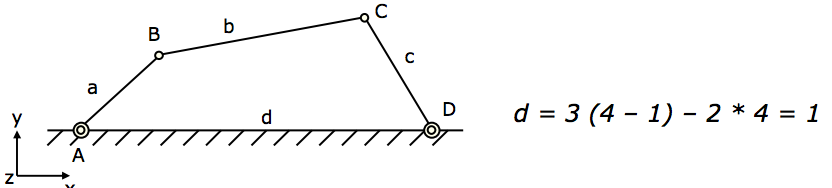
\includegraphics[width=.8\linewidth]{grubler.png}
\caption{Exemple de calcul de d.d.l avec Grübler}
\label{grubler}
\end{figure}

{\color{red}MAIS} Grübler ne marche que dans le cas des problèmes {\color{orange}plan} (2D) et ne tient pas compte cas de {\color{orange}contraintes non indépendantes} (ex : la boucle prismatique ) ou encore des cas de variation {\color{orange}locale} ou {\color{orange}globale} du nombre de ddl (ex: Le 3-barres + béquille)\\

\subsection*{3. Mécanismes à couples inférieurs – articulés}
{\color{orange}Système articulé} (2D ou 3D) – domaine des {\color{orange}mécanismes} $\Rightarrow$ uniquement couples {\color{orange}R}, {\color{orange}P} et {\color{orange}S} (non-dégénérés)\\
$\Leftrightarrow$\\
Système articulé (2D ou 3D) – domaine des systèmes {\color{orange}multicorps} $\Rightarrow$ tous couples confondus (aussi les dégénérés)\\

Mécanismes plans - trois-barres $\Rightarrow$ Manivelle ou balancier ? (regarder figure \ref{grubler})\\
Conditions de Grashof:\\
\begin{itemize}
\renewcommand{\labelitemi}{$\bullet$}
\item{\begin{tabbing}
a est manivelle si, simulta\=nément :\\
\> $d+a\leq b+c$\\
\> $|d-a|\geq|b-c|$\\
\end{tabbing}}
\item{\begin{tabbing}
a et c sont manivelles si d\=e plus :\\
\> $d+c\leq b+a$\\
\> $|d-c|\geq|b-a|$\\
\> $\Rightarrow d\leq b$\\
\end{tabbing}}
\end{itemize}

{\color{orange}Positions de bifurcation} $\Rightarrow$ Le mouvement imposé à un organe déterminé peut {\color{orange}cinématiquement} entraîner {\color{orange}plusieurs mouvements distincts} d’autre organes\\
$\bullet$ Accroissement local du nombre de ddl\\
$\bullet$ Déficience locale d’actionnement\\
$\Rightarrow$ Une bifurcation est “ actionneur-dépendant ” $\Rightarrow$ Changer d'actionneur ( organe du mécanisme qu'on actionne) peut résoudre le problème de bifurcation\\

Autre solution au problème de bifurcation: le suractionnement\\
$\bullet$ Plus d'actionneurs que “ normalement ” nécessaire\\

{\color{orange}Théorème d’équivalence} $\Rightarrow$ La trajectoire réalisée par un point attaché à la bielle b d’un trois barres peut être réalisée à partir de deux autres trois-barres équivalents quant à cette trajectoire (théorème de Roberts-Chebyshev)\\

Bielle-manivelle:

\begin{figure}[H]
\centering
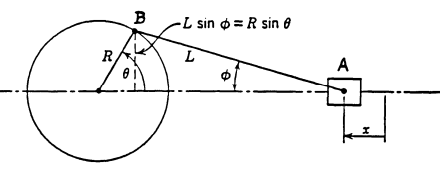
\includegraphics[width=.8\linewidth]{biellemanivelle.png}
\caption{Mécanisme de bielle-manivelle}
\label{manivelle}
\end{figure}

\begin{bluebox}
\begin{tabbing}
tttttttttttttttttttttttt\=tttttttttttttttttttttttttttttttttttttttt\=ttttttt\=ttttttt\=ttttttttttttttttttttt\kill
Déplacement de A:\\
\>$x_A=R(1-\cos\theta)+L\{1-(1-\dfrac{R^2}{L^2}\sin^2\theta)^{1/2}\}$\\\\
$x_A$ fonction périodique de $\theta$ $\Rightarrow$ développement série de Fourier – troncature $2^{\text{ème}}$ ordre)\\
$x_A=R(1-\cos\theta)+\dfrac{R^2}{2L}\sin^2\theta$\>\>$R<<L$\>\>$(\dfrac{L}{R}>3.5)$\\\\
Vitesse de A:\\
$v_A=R\omega\sin\theta$\>\>\>$v_{max}=R\omega$\\\\
Accélération de A:\\
$a_A=R\omega^2\cos\theta$
\end{tabbing}
\end{bluebox}\\\\

Fonction mécanisée de l’homothétie: Pantographe (mécanisme à 2 d.d.l):

{\color{orange}Homothétie} de centre O (fixe) et de rapport K = transformation géométrique qui fait correspondre à tout point M un point M’ tel que OM’ = K OM
$\Rightarrow$ pantographe permet de reproduire des mouvement par homothétie\\

Mécanisme dans l'espace: joint de cardan (1 d.d.l + “1”):

$\Rightarrow$ Accouplement {\color{orange}flexible} à éléments rigides entre arbres concourants\\
\begin{itemize}
\renewcommand{\labelitemi}{$\bullet$}
\item{Accepte les mêmes déformations angulaires qu’une rotule (lim. $\alpha_{max}$)}
\item{Transmission d’un couple entre les 2 arbres (input en D, output en C)}
\item{Angle $\alpha$ non nul et variable entre leurs axes (= un « second » ddl)}
\item{{\color{red}Inconvénient} : Transmission non homocinétique}\\
\end{itemize}

\begin{bluebox}
\begin{tabbing}
ttttt\=ttttttttttttttt\=ttttttttttttttt\=tttttttttttttttt\=tttttttttttttttttttttttttttttttttttttttttttttttt\kill
\>$\omega_{in} constant$\>\>$\Rightarrow$\>$\omega_{out}variable$\\\\
\>\>$\dfrac{\omega_2}{\omega_1}=\dfrac{\cos\alpha}{1-\sin^2\theta_1\sin^2\alpha}$
\end{tabbing}
\end{bluebox}\\\\

{\color{blue}SOLUTION}: joint de cardan {\color{orange}double}\\
$\rightarrow$ Deux joints consécutifs d’angle $\beta$ = $\alpha$/2\\
$\rightarrow$ Fourches de l’arbre intermédiaire dans un même plan\\

$\Rightarrow$ En pratique, on le veut toujours homocinétique!\\
Il existe d'autre type de joint homocinétique (comme joint à billes)\\
Transmission entre 2 axes parallèles mais décalés $\Rightarrow$ joint d'Oldham\\

\subsection*{4. Mécanismes à couples supérieurs}
{\color{orange}Couples inférieurs $\Leftrightarrow$ Couples supérieurs}\\

{\color{orange}Nature du contact}\\
$\bullet$ Surface pour C.I. \\
$\bullet$ Point / ligne pour C.S.\\ 
$\Rightarrow$ répercussion sur la grandeur des efforts transmissible\\
{\color{orange}Type de mouvement}\\
$\bullet$ Glissement (entre les surfaces) pour C.I. (glissière, tourillon, …) \\
$\bullet$ Roulement, Roulement/Glissement ou Glissement pour les C.S \\
{\color{orange}Et donc} :\\
$\bullet$ C.I. pour machines de « grande » puissance – pertes par frottement, usure \\
$\bullet$ C.S. pour mécanismes haut rendement, de précision (usure moindre)\\
$\Rightarrow$ accroissement de l’effort transmissible par multiplication des contacts\\

{\color{orange}Fonctions}\\
$\bullet$ Guidage : cames, coulisses, leviers, …mouvement alternatif, glissement, irréversibilité\\
$\bullet$ Transmission : roues de friction et engrenages\\

\underline{Système de guidage:}\\
{\color{orange}Satisfaire une loi de mouvement (organe conduit)} $\Rightarrow$ “ Fonction mécanisée le long d’une trajectoire ”\\
Un point P (matériel) de l’organe mené :\\
- parcourt une trajectoire p imposée,\\
- tout en suivant une surface s ou une ligne c de l’organe menant\\

$\Rightarrow$ Came-Follower\\

\underline{Mécanismes à roulement plan:}\\
Trains de roulement $\Rightarrow$ Plusieurs couples de roulement en série\\

\begin{bluebox}
\begin{tabbing}
tttt\=tttttttttttttttttttt\=ttttttttttttttttttttttttttttt\=ttttttttttttttttttttttttttttttttttttttttttttttt\kill
Profils circulaires – rapport de transmission (avec 2 profils):\\
\>$\vec{\omega}=\omega\vec{I}_3$\>$\vec{\omega'}=\omega'\vec{I}_3$\\
\>$\dfrac{\omega'}{\omega}>0$\>lorsque $\vec{\omega'}\cdot\vec{\omega}>0$\>Roulement {\color{orange}intérieur} (roue dans roue)\\\\
\>$\dfrac{\omega'}{\omega}<0$\>lorsque $\vec{\omega'}\cdot\vec{\omega}<0$\>Roulement {\color{orange}extérieur} (roue contre roue)\\\\
$\Rightarrow \dfrac{\omega'}{\omega} = \pm \left|\dfrac{r}{r'}\right|$\>\>- : roulement extérieur\>+ : roulement intérieur
\end{tabbing}
\end{bluebox}\\\\

{\color{orange}Cas étudiés}\\
$\bullet$ Corps de base (châssis) : mobile à vitesse angulaire $\Omega$ autour de son c.i.r.\\
$\bullet$ Profils : profils circulaires articulés à entraxes constants (hypothèse)[entraxe : $d=r+r'$]\\
$\bullet$ Roues : numérotées de 1 à n , vitesses angulaires absolues $\omega_1,…, \omega_n$\\
$\bullet$ Rayons des roues 2 à n-1:2 rayons notés r’ (récepteur) et r’’ (moteur)\\

\begin{bluebox}
\begin{tabbing}
tttt\=tttttttttttttttttttt\=ttttttttttttttttttttttttttttt\=ttttttttttttttttttttttttttttttttttttttttttttttt\kill
Trains de roulement : Contact de 2 roues sur le châssis mobile:\\
$\dfrac{\omega_2-\Omega}{\omega_1-\Omega} = \pm \left|\dfrac{r_1}{r_2}\right|$\>\>- : roulement extérieur\>+ : roulement intérieur\\\\
Train complet$\Rightarrow$“ {\color{orange}formule de Willis} ”:\\
$\dfrac{\omega_n-\Omega}{\omega_1-\Omega} = (-1)^p\dfrac{r_1}{r_2'}\dfrac{r_2''}{r_3'}\cdots\dfrac{r_{n-1}''}{r_n}$\>\>\>“produits r. moteurs / produits r. récepteurs”\\
$\Rightarrow$ 2 d.d.l\>\>\> p = nombre de couples “ extérieurs ” \begin{tikzpicture}
\draw[color=orange] (0, 0) circle (.3);
\draw[color=orange] (0.5, 0) circle (.2);
\end{tikzpicture}
\end{tabbing}
\end{bluebox}\\\\

Un train {\color{orange}épicycloïdal} (ou planétaire) est un train de roulement tel que :\\
$\bullet$ La première roue et le châssis tournent autour d’un même axe fixe\\
$\bullet$ (en général), la dernière roue n tourne aussi autour cet axe (roues récurrentes)\\
$\Rightarrow$ Boîte de sur- ou de dé-multiplication\\

Pour calculer le rapport entre $\omega_{in}$ et $\omega_{out}$ $\Rightarrow$ {\color{orange}Willis}\\
Si plusieurs châssis ($n$ châssis) alors plusieurs Willis ($n$ Willis)\\

\underline{Roulement dans l’espace:}\\
Couples de roulement {\color{orange}coniques} :\\
$\Rightarrow$ Transmission par roulement de cônes de révolution entre 2 axes concourants a et a’\\

\begin{bluebox}
\begin{tabbing}
tttt\=tttttttttttttttttttt\=ttttttttttttttttttttttttttttt\=ttttttttttttttttttttttttttttttttttttttttttttttt\kill
Rapport de transmission $\Rightarrow$ comme le cas plan:\\
$\dfrac{\omega'}{\omega} = \pm \left|\dfrac{r}{r'}\right|$\>\>- : roulement extérieur\>+ : roulement intérieur\\\\
Ou encore:\\\\
$\dfrac{\omega'}{\omega} = \dfrac{\sin\gamma}{\sin\gamma'}$\>\>$\gamma+\gamma'=\Gamma$\\
\>\>$\Gamma$ = l'angle entre les 2 axes concourants a et a'
\end{tabbing}
\end{bluebox}\\\\

{\color{orange}Trains de roulement dans l’espace} = Succession de contacts coniques de même sommet : 2 cas\\
$\bullet$ 1)Par nécessité : quand $\Gamma$ devient très (« trop ») grand\\
$\Rightarrow$ exemple : $\Gamma$ = $180^\circ$ inversion de sens de rotation in/out – rapport donné\\
$\bullet$ Par choix : application particulière: différentiel\\

\begin{bluebox}
\begin{tabbing}
tttt\=ttttttttttttttttt\=tttttttttt\=tttttttttttttttttttttt\=ttttttttttttttttttttttttttttttttttttttttttttttt\kill
$\dfrac{\omega_3-\Omega}{\omega_1-\Omega} = -\dfrac{\sin\gamma_1}{\sin\gamma_3}$\>\>\>\>$\Omega$ carter du différentiel\\\\
\>\>$\Rightarrow \Omega = \dfrac{\omega_1\sin\gamma_1+\omega_3\sin\gamma3}{\sin\gamma_1+\sin\gamma_3}$\\\\
Cas particulier $\gamma_1=\gamma_3(= 45^\circ)$ : différentiel\\\\
\>\>\>$\Omega = \dfrac{\omega_1+\omega_3}{2}$
\end{tabbing}
\end{bluebox}\\\\

\underline{Variateurs}\\
$\bullet$ Roues de frictions versus engrenages\\
{\color{green}+ Acceptent des variations de rayons $\Rightarrow$ variation continue de vitesse}\\
{\color{red}- faibles puissances transmises}\\

\subsection*{5. Engrenages}
Roues cylindriques / coniques (“ roues à friction ”) $\Rightarrow$ Inconvénient majeur : limitation de l’effort transmis\\
{\color{green}Solution} $\Rightarrow$ Modification de forme (des profils) $\Rightarrow$ {\color{orange}Engrenages} : Cames à profils périodiques\\

Rapport identique à celui de 2 roues de friction de rayons donnés $\Rightarrow$ 2 cercles primitifs (général : courbe primitive)\\

\begin{bluebox}
\begin{tabbing}
tttt\=tttttttttttttttttttt\=ttttttttttttttttttttttttttttt\=ttttttttttttttttttttttttttttttttttttttttttttttt\kill
Vitesse points matériels $M_1$, $M_2$:\\
\>$\bullet$ différentes tangentiellement (… glissement)\\
\>$\bullet$ égales suivant n (pas de pénétration) et donc :\\\\
\>$(\vec{\omega}_1\times O_1\vec{M})\cdot M\vec{P} = (\vec{\omega}_2\times O_2\vec{M})\cdot M\vec{P}$\\\\
\> $\Rightarrow \omega_1O_1P=\omega_2O_2P$\\\\
$\Rightarrow$ Pour un rapport {\color{orange}constant}, P doit être fixe
\end{tabbing}
\end{bluebox}\\\\

\begin{orangebox}
{\color{orange}Condition fondamentale d’engrènement} :\\
Les profils en prise sont tels qu’à tout moment la normale commune au point de contact (M) passe par un point P, fixe, point de tangence des cercles primitifs
\end{orangebox}\\\\

\begin{bluebox}
\begin{tabbing}
ttttttttttttt\=tttttttttttttttttttttttttttttttttttttttttttttttttt\=ttttttttttttttttttttttttttttttttttttt\kill
Glissement au contact: \\
\> $|v_g|=(|\omega_1|+|\omega_2|)PM$\> Dentures {\color{orange}extérieures}\\
\> $|v_g|=(|\omega_1|-|\omega_2|)PM$\> Dentures {\color{orange}intérieures}\\\\
\begin{orangebox}
PM doit rester limité $\Rightarrow$ “ bcp de petites dents ”
\end{orangebox}
\end{tabbing}
\end{bluebox}\\\\

$\Rightarrow$ “ Willis ” d’application en utilisant les cercles primitifs\\

\begin{orangebox}
\begin{tabbing}
Dentures : \=caractéristiques:\\
\> Cercle de pied, de tête $\Rightarrow$ limite « physique » des dents\\
\> Addendum $\Rightarrow$ hauteur de tête $h'$\\
\> Dedendum $\Rightarrow$ hauteur de pied $h''$\\
\> Hauteur de dent $\Rightarrow h = h' + h''$\\
\> Jeux de fond $\Rightarrow h_1''-h_2'$ \& $h_2''-h_1'$\\
\> Engrènement “ matériellement ” possibl\=e si :\\
\>\>$h_1'\leq h_2''$ \& $h_2'\leq h_1''$\\
\> Nombres de dents $\Rightarrow$ $z$\\
\> Epaisseur des dents (mesurée sur primitive) $\Rightarrow$ $a$\\
\> Pas ” p “ [m] $\Rightarrow p = \dfrac{2\pi|R_1|}{z_1}= \dfrac{2\pi|R_2|}{z_2}$\\
\> Module “ m ” [mm] $\Rightarrow m = \dfrac{2R}{z} = \dfrac{p}{\pi}$\\
\> Eviter coincement $\Rightarrow a_1+a_2<p$\\
\> Jeu circonferentiel $\Rightarrow j = p-(a_1+a_2)$\\
\> Ligne de contact LC (“d’engrènement”) $\Rightarrow$ Lieu points géométriques de contact\\
\> Arc \=d’engrènement AE [m] $\Rightarrow$\\
\>\>Arc, compté sur le(s) cercle primitif correspondant à la durée d’un contact\\
\>Coefficient de recouvrement k $\Rightarrow k = \dfrac{AE}{p}$, entre 1.3 et 2\\
\> Variante $p_b$ et $k_b$ de p et b avec r (c. de base) au lieu de R (c. primitif)
\end{tabbing}
\end{orangebox}\\\\

\underline{Dentures à développante de cercle:}\\
{\color{orange}Définition} : Forme générée par un point matériel d’une droite qui roule sans glisser sur un cercle\\

{\color{orange}Avantages} (en résumé):\\
$\bullet$ Profils conjugués et assortis (de facto)\\
$\bullet$ Invariance du rapport de transmission (si ~ entraxe)\\
$\bullet$ Angle de pression $\alpha$ constant pendant l’engrènement\\

{\color{orange}Interferérence}:\\
$\bullet$ Prolongement du profil en dessous du cercle de base (endroit où la développante est non définie) : se fait suivant un Rayon (en pratique)\\

\underline{Engrenages dans l’espace:}\\
Dentures {\color{orange}hélicoïdales} (axes $\parallel$):\\
“ Denture droite qui a subi une torsion suivant l’axe ” $\Rightarrow$ s’obtient par le déplacement du profil (développante dans un mouvement hélicoïdal $\Leftrightarrow$ hélice circulaire d’angle $\beta’$ (max. $15^\circ$)\\
Mise en contact {\color{orange}progressif} des dents $\Rightarrow$ bruit réduit\\

\begin{orangebox}
\begin{tabbing}
Caractéristiq\=ue d'engrenages hélicoïdales:\\
\> Largeur de l'engrange $\Rightarrow$ b\\
\>Recouvrement total $\Rightarrow k_t = \dfrac{q+s_b}{p_b}=k+\dfrac{s_b}{p_b}$\\
\> Longueur d’engrènement correspondant à la durée d’un contact $\Rightarrow q$\\
\> Saut de base $s_b \Rightarrow$ déport de la droite de contact entre sections extrèmes dans\\
\>le plan d’engrènement $\Rightarrow s_b = b\tan\beta'$\\
\> Longueur maximale de contact $\Rightarrow l_{max} = \dfrac{b}{\cos\beta'}$
\end{tabbing}
\end{orangebox}\\\\

Plus de recouvrement $\Rightarrow$ Longueur de contact plus grande $\Rightarrow$ efforts transmissibles accrus\\
Nombre minimum de dents réduit\\
{\color{red}MAIS} Poussée axiale par rapport à engrenages droits\\

\subsection*{6. Le Frottement}
Assemblages fixes $\Rightarrow$ couples inférieurs $\Rightarrow$ {\color{orange}utilisent} les frottements\\
Assemblages mobiles $\Rightarrow$ couples inférieurs et supérieurs $\Rightarrow$ {\color{orange}redoutent} les frottements (lubrification)\\

{\color{orange}Transmission}: Organe qui transmet de l’énergie mécanique d’une partie  d’un ensemble mécanique à une autre (transmission entre « sous-systèmes mécaniques)\\
$\Rightarrow$ On recherche le plus haut rendement possible\\
{\color{orange}Accouplement} : cas particulier de la transmission coaxiale d’un arbre à l’autre (rigide [bride,...] ou élastique [courroie,...])\\

Forces de {\color{orange}frottement} : 2 corps en contact surfacique, mouvement relatif entre eux $\Rightarrow$ Forces tangentielles résistantes au niveau de la surface\\
$\bullet$ Utile: on s'appui sur cette force (marcher, freiner,...)\\
$\bullet$ Nuisible: dissipation d'énergie, usure\\

\underline{Forttement sec:}\\
Deux corps, pas de lubrification\\

\begin{bluebox}
\begin{tabbing}
ttttttttttttt\=tttttttttttttttttttttttttttttttttttt\=ttttttttttttttttttttttttttttttttttttttttttttttttttt\kill
Frottement en mouvement: \\
\> $T=fN$\>$T$ et $N$ : tangentielle et normale (résultante)\\
\>\>f : coefficient de frottement {\color{orange}cinétique}\\\\
Frottement statique:\\
\>$T_{max}=f_0N$\>$T_{max}>T$\\
\>\>$f_0 (>f)$: coefficient de frottement {\color{orange}statique}\\\\
Angle de frottement:\\
\> $\dfrac{T}{N}=\tan\phi=f$\>$\dfrac{T_{max}}{N}=\tan\phi_0=f_0$
\end{tabbing}
\end{bluebox}\\\\

\underline{Frottement visqueux:}\\
Deux corps et lubrifiant (troisième corps [graisse, huile, air,...])\\

\begin{center}
\begin{tabular}{l||r}
{\color{orange}Frottement sec (“ immédiat ”)}&{\color{orange}Frottement visqueux (“ médiat ”)}\\
\hline
$T$ fonction de $N$&$T$ indépendant de $N$\\
$T$ indépendant de la vitesse&$T = k.v$\\
$T$ indépendant de l’aire&$T = k’. aire$\\
$T$ dépendant de la rugosité&$T$ indépendant de la rugosité
\end{tabular}
\end{center}
\begin{orangebox}
Phénomène (et donc modèles) tout à fait différent (s)
\end{orangebox}\\\\

\noindent$\bullet$ Lubrification hydrodynamique (ou hydrostatique) : paliers lisses lubrifiés, butées) \\
$\Rightarrow$ Le film sépare complètement les corps : aucun contact, {\color{orange}aucune usure}\\
$\bullet$ Lubrification mixte (ex. contact piston-segment-chemise aux points morts haut et bas)\\
$\Rightarrow$ contact intermittent des aspérités - action hydrodynamique partielle, {\color{orange}peu d'usure}\\
$\bullet$ Lubrification frontière : pour petits mécanismes (gond, charnière, serrure..)\\
$\Rightarrow$ graissage (plutôt que lubrification) pour réduction d’usure\\

\underline{Résistance au roulement}\\
pourquoi cette résistance alors que $T=0$?\\
$\bullet$ Contact non ponctuel $\Rightarrow$ OK mais pas suffisant\\
$\bullet$ Déformation alternée locale du matériau \\
$\rightarrow$  se comptine devant et se détend derrière\\
$\rightarrow$ Force “ de compression ” > Force de “ détente ” $\Rightarrow$ couple retardateur\\
Mais ce $T_r$ rien du tout par rapport ) $fN$\\

$\Rightarrow$ La roue = excellente invention\\

\subsection*{7. Glissement par translation}
Mise en situation : Bloc de poids $P = mg$ sur plan incliné $\alpha$\\
$\rightarrow F = P\sin\alpha$\\
$\rightarrow N = P\cos\alpha$\\
$\Rightarrow$ Bloc à l'arrêt si $\alpha\leq\phi_0$ ($F=N\tan\alpha$ et angle frottement $f_0=\tan\phi_0$)\\ 
$\Rightarrow$ Mouvement si $\alpha>\phi_0 \Rightarrow P\cos\alpha\tan\phi_0<\sin\alpha$\\

Pour remonter le bloc, quel effort choisir? {\color{orange}Parallèle} ou {\color{orange}horizontal}?\\
\begin{bluebox}
\begin{tabbing}
ttttttttttttt\=tttttttttttttttttttttttttttttttttttt\=ttttttttttttttttttttttttttttttttttttttttttttttttttt\kill
Parallèle : $F_{ext}$ :\\
\> $F_{ext}'=\dfrac{P\sin(\alpha+\phi_0)}{\cos\phi_0}$\>début démarrage vers le haut\\
\> $F_{ext}''=\dfrac{P\sin(\alpha-\phi_0)}{\cos\phi_0}$\>début démarrage vers le bas\\\\
Horizontal : $H_{ext}$ :\\
\> $H_{ext}'=\tan(\alpha+\phi_0)$\\
\> $H_{ext}''=\tan(\alpha-\phi_0)$\\\\
Rendement:\\
\>$\eta_{F_{ext}}=\dfrac{\sin\alpha\cos\phi}{\sin(\alpha+\phi})$\\
\>$\eta_{H_{ext}}=\dfrac{\tan\alpha}{\tan(\alpha+\phi})$\\\\
\>$\Rightarrow$ Rendement max de $H_{ext}$ pour $\alpha = 42^\circ$
\end{tabbing}
\end{bluebox}\\\\

\begin{bluebox}
\begin{tabbing}
ttttttttttttt\=tttttttttttttttttttttttttttttttttttt\=ttttttttttttttttttttttttttttttttttttttttttttttttttt\kill
Vis sans fin avec charge $Q$:\\
Couple $T$ à appliquer et couple idéale sans frottement $T_\circ$:\\
\> $T = \dfrac{Qd}{2}\tan(\alpha+\phi)$\\\\
\> $T_\circ = \dfrac{Qd}{2}\tan\alpha$\\
Rendement :\\
\>$e=\dfrac{T_\circ}{T} = \dfrac{\tan\alpha}{\tan(\alpha+\phi)} (= \dfrac{QL}{2\pi T}) $
\end{tabbing}
\end{bluebox}\\\\

Il est important que l'assemblage ne se desserre pas “ naturellement ” (par exemple action de $g$) $\Rightarrow$ On prend $\alpha < \phi$\\

\underline{Glissement dans une rainure:}\\
\begin{bluebox}
\begin{tabbing}
ttttttttttttt\=tttttttttttttttttttttttttttttttttttt\=ttttttttttttttttttttttttttttttttttttttttttttttttttt\kill
\> $N=\dfrac{P}{2\cos\beta}$\>$2\alpha$ = angle de la rainure\\
\> $T = f_0N = \dfrac{F_0P}{2\cos\beta}$\>$\beta = \pi/2-\alpha$\\
\> $F = 2T = \dfrac{F_0P}{\cos\beta}$\\
Coefficient de frottement :“ majoré ” (par rapport à P $\perp$ contact):\\
\>$f' = \dfrac{f}{\cos\beta}=\dfrac{f}{\sin\alpha}$\\\\
$\Rightarrow$ Rainure : accroissement “ {\color{orange}artificiel} ” du coefficient de frottement
\end{tabbing}
\end{bluebox}\\\\

{\color{orange}Arc-boutement} d’un mécanisme :Dans une positon donnée, un effort, aussi grand soit-il , ne peut provoquer le mouvement cinématique de celui-ci.\\

\subsection*{8. Glissement par rotation relative}
\underline{Clavettes et goupilles ({\color{orange}démontable}):}\\
$\bullet$ Assemblage(s) avec pièce supplémentaire\\
$\bullet$ Empêcher le glissement de translation et/ou de rotation entre deux organes\\
$\bullet$ Résiste à des sollicitations tendant à disjoindre l’assemblage par {\color{orange}cisaillement de sections} transversales à la clavette\\
$\bullet$ L’angle $\alpha$ (“ tapered pin ”) assure un {\color{orange}serrage} parallèle au cisaillement\\
$\bullet$ Desserrage “ dynamique ” évité par goupille ou écrou (goupille pour bloquer goupille, oui...)\\

\begin{bluebox}
\begin{tabbing}
ttttttttttttt\=tttttttttttttttttttttttttttttttttttt\=ttttttttttttttttttttttttttttttttttttttttttttttttttt\kill
Dimensionnement au cisaillement des sections transversales:\\
\>$M_t=S\cdot D\cdot\tau_{adm}$\> $M_t$ = Couple transmissible\\
\>\>$S$ = section goupille\\
\>$D$ = diamètre de l'axe\>$\tau_{dam}$ = contrainte de cisaillement admissible\\\\
Clavette longitudinale : dimensionnement (longeur $L$, largeur $d/4$, axe diamètre $d$):\\
\>$M_t = \dfrac{\tau_{adm}Ld^2}{8}$
\end{tabbing}
\end{bluebox}\\\\

Rivet: même principe, mais {\color{orange}non démontable}\\
$\bullet$ Une tête existe, deuxième formé à l'assemblage (rivetage)\\

\underline{Frottement dans les paliers}\\
Machine tournante $\Leftrightarrow$ arbre $\Leftrightarrow$ {\color{orange}paliers}\\
{\color{orange}Palier lisse} “ journal bearing ” :\\
$\bullet$ surfaces cylindriques\\
$\bullet$ charge transversale\\
{\color{orange}Tourillon} : portée de l’arbre qui fait contact\\
{\color{orange}Coussinet} (ou moyeu) : portée du palier qui fait contact\\
$\bullet$ surfaces de contact cylindriques\\
$\bullet$ charge transversale F\\

\begin{orangebox}
\begin{tabbing}
ttttttttttttt\=tttttttttttttttttttttttttttttttttttttttttttttttttttttttt\=ttttttttttttttttttttttttttttttt\kill
Forces – configuration en mouvement:\\
$f = 0$: \> Resultante $R$ et normale $N$ alignées, passent par centre palier $O$\\
$f \neq 0$:\> $R$ incliné de $\phi$ par rapport à $N$\\
\> $R$ (= poids $P$) tangent cercle de rayon $p$ \\
\> $\Rightarrow$ {\color{orange}cercle de frottement} $=$ lieu de tangence des efforts réciproques entre les organes\\
\> Couple résistant $M=Rp$\\
\> Puissance dissipée $P_{diss} = M\omega=Mp\omega$\\\\
L'arbre “grimpe” dans son palier en régime
\end{tabbing}
\end{orangebox}\\\\

\begin{bluebox}
\begin{tabbing}
ttttttttttttt\=tttttttttttttttttttttttttttttttttttt\=tttttttttttttttttttt\=ttttttttttttttttttttttttttttttt\kill
Equilibre en régime :\\
\>$R=P$\\
\>$C_{moteur}-C_r=M=Rp$\> $C_r$ = charge\\
\>$p=r\sin\phi\approx fr$\> $r$ = rayon arbre\\\\
Dire que $f$ est ponctuel $\Rightarrow$\> \>Envisager $p=fr \rightarrow p=f_ar$\\
\>Répartition uniforme (cas défavorable):\>\>$f_a=f\pi/2$\\
\>Répartition parabolique (cas vraisemblable):\>\>$f_a=f4/\pi$
\end{tabbing}
\end{bluebox}\\\\

\underline{Utilisation du cercle de frottement}\\

\begin{figure}[H]
\centering
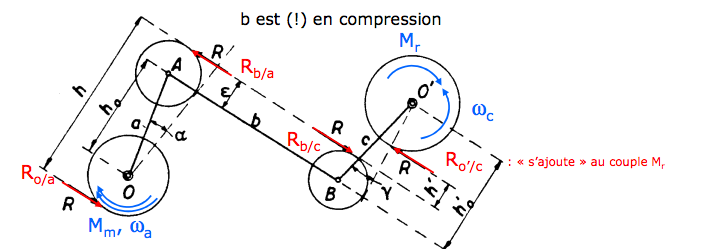
\includegraphics[width=\linewidth]{cerclef.png}
\caption{Utilisation du cercle de frottement}
\label{cerclef}
\end{figure}

\begin{bluebox}
\begin{tabbing}
ttttttttttttt\=tttttttttttttttttttttttttttttttttttt\=tttttttttttttttttttt\=ttttttttttttttttttttttttttttttt\kill
Rendement:\\
\>$\eta = 1-f_a(\dfrac{r_o+r_A}{a\cos\alpha}+\dfrac{r_o'+r_B}{c\cos\gamma})$\\\\
\>$\eta = \dfrac{h'/h}{h_o'/h_o}$\\\\
\begin{orangebox}
Le rendement sera élevé lorsque $\alpha$ et $\gamma$ sont proches de 0\\
$\eta$. = 0 dans certaines positions (ex. h’=0) $\Rightarrow$ détermine les {\color{orange}angles morts} 
\end{orangebox}
\end{tabbing}
\end{bluebox}\\\\

\underline{Freins à sabot - à segments (pas connaitre):}\\

\begin{bluebox}
\begin{tabbing}
ttttttttttttt\=tttttttttttttttttttttttttttttttttttt\=tttttttttttttttttttt\=ttttttttttttttttttttttttttttttt\kill
Force à appliquer:\\
\>Sabot pivote autour de $A$, à $c.\vec{x}$ et $a.\vec{y}$ du centre $O$ du disque à freiner\\
\>$F$ appliquer à $b.\vec{x}$ de $A$\\
\>Disque de rayon $r$ et moment de freinage $M$\\
\>$F=[c\pm f(a-c)]\dfrac{M}{bfr}$\> "$-$" si rotation “vers” $A$
\end{tabbing}
\end{bluebox}\\\\

\underline{Plateaux d’accouplement:}\\

\begin{bluebox}
\begin{tabbing}
ttttttttttttt\=tttttttttttttttttttttttttttttttttttt\=tttttttttttttttttttt\=ttttttttttttttttttttttttttttttt\kill
Couple maximal transmissible :\\
\>$M_{max}=\dfrac{2}{3}fnF\dfrac{r^3_2-r^3_1}{r^2_2-r^2_1}$\> $n$ = nombre de boulon, $F$ = force de serrage\\\\
\>$r_m = \dfrac{2}{3}\dfrac{r^3_2-r^3_1}{r^2_2-r^2_1}$\>Effort de serrage $P=nF$\\\\
\>$M_{max}=fPr_m$
\end{tabbing}
\end{bluebox}\\\\

\underline{Paliers de butée (« crapaudine »):}\\

\begin{bluebox}
\begin{tabbing}
ttttttttttttt\=tttttttttttttttttttttttttttttttttttt\=tttttttttttttttttttt\=ttttttttttttttttttttttttttttttt\kill
Couple maximal transmissible :\\
\>$M_{max}=\dfrac{2}{3}fnF\dfrac{r^3_2-r^3_1}{r^2_2-r^2_1}$\\
Effort axial P sur arbre:\\
\>$P = 2\pi C(r_2-r_1)$\>$C$ est une constante: $C=pr$\\
Moment résultant (résistant) :\\
\>$M=fP\dfrac{r_1+r_2}{2}$
\end{tabbing}
\end{bluebox}\\\\

\underline{Embrayage à disque (rigide):}

\begin{bluebox}
\begin{tabbing}
ttttttttttttt\=tttttttttttttttttttttttttttttttttttt\=tttttttttttttttttttt\=ttttttttttttttttttttttttttttttt\kill
Rappel :\\
\>$M=fP\dfrac{r_1+r_2}{2}$\>$P = 2\pi C(r_2-r_1)$\\\\
\underline{Embrayage}: $F\Leftrightarrow P$, $p\Leftrightarrow p_{max}$(pression) $\Rightarrow$ n contacts :\\\\
\>$M_{max}=nfF\dfrac{r_1+r_2}{2}$\>$P = 2\pi (p_{max}r_1)(r_2-r_1)$\\\\
\>\>$r_{1_{opt}}=\dfrac{r_2}{\sqrt{3}}$
\end{tabbing}
\end{bluebox}\\\\

\underline{Embrayage à disque (flexible):}

\begin{bluebox}
\begin{tabbing}
ttttttttttttt\=tttttttttttttttttttttttttttttttttttt\=tttttttttttttttttttt\=ttttttttttttttttttttttttttttttt\kill
Couple maximal transmissible :\\
\>$M_{max}=\dfrac{2}{3}fnF\dfrac{r^3_2-r^3_1}{r^2_2-r^2_1}$\> $n$ = nombre de contacts
\end{tabbing}
\end{bluebox}\\\\

\underline{Frein à disque:}

\begin{bluebox}
\begin{tabbing}
ttttttttttttt\=tttttttttttttttttttttttttttttttttttt\=tttttttttttttttttttt\=ttttttttttttttttttttttttttttttt\kill
Couple de freinage :\\
\>$M=2fP\dfrac{r_1+r_2}{2}$
\end{tabbing}
\end{bluebox}\\\\

\subsection*{9. Liens flexibles}

$\Rightarrow$ Etude de l’{\color{orange}adhérence} et du {\color{orange}glissement} par rotation entre :\\
$\bullet$ Un corps rigide (tambour, poulie, …, pignon)\\
$\bullet$ Un corps flexible appelé {\color{orange}lien}\\
$\rightarrow$ Exigences géométriques faibles \\
$\rightarrow$ Pas de lubrification\\
$\rightarrow$ Rapport de transmission {\color{orange}quasi} constant (mais beaucoup d’applications)\\

{\color{orange}Courroies}: plates ou crantées (pas de glissement), rectangulaire ou trapèzoïdale [en “V”] ($f'=f/\cos\beta$)\\

\begin{bluebox}
\begin{tabbing}
ttttttttttttt\=ttttttttttttttttttttttttttt\=ttttttttt\=tttttttttttttttttttt\=ttttttttttttttttttttttttttttttt\kill
Calcul de la tension :\\
\>$t=pr$\>\>$t$ = tension et $p$ = force de pression\\\\
\>\>$\ln\dfrac{t}{T_0}=f(\theta-\theta_0)$\\\\
Pour une poulie avec {\color{blue}$T_0$} la “ {\color{blue}sortie} ” de la poulie (côté “ lâche ”) et {\color{green}$T_1$}“ {\color{green}l'entrée} ” (côté \\
“ tendu ”)[angle $\alpha$ entre $T_0$ et $T_1$] $\Rightarrow$ \\\\
\>\>$T_1 = T_0e{f\alpha}$\\\\
Moment $M$ appliqué au tambour (rayon $r$):\\
\>\>$M=(T_1-T_0)r$
\end{tabbing}
\end{bluebox}\\\\

\underline{Frein differentiel :}\\
\begin{minipage}[c]{.4\linewidth}
\begin{figure}[H]
\centering
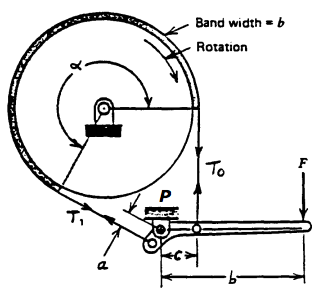
\includegraphics[width=0.8\linewidth]{frein.png}
\caption{Frein differentiel}
\label{frein}
\end{figure}
\end{minipage}
\hfill
\begin{minipage}[c]{.5\linewidth}
\begin{bluebox}
\begin{tabbing}
ttttttttttttt\=ttttttttttttttttttttttttttt\=ttttttttt\=tttttttttttttttttttt\=ttttttttttttttttttttttttttttttt\kill
Calcul de la tension :\\
$F$ nécessaire au freinage:\\
\>$F = \dfrac{T_0c-T_1a}{b} = \dfrac{Mf}{br}\dfrac{c-ae^{f\alpha}}{e^{f\alpha}-1}$\\\\
Si $a=0$: frein simple:\\
\>$F=\dfrac{T_0c}{b}$\\
Si $a\neq0$: frein différentiel:\\
\>$T_1$ réduit $F$ nécessaire
\end{tabbing}
\end{bluebox}
\end{minipage}\\\\

\underline{Adhérence des liens flexibles:}\\

\begin{bluebox}
\begin{tabbing}
ttttttttttttt\=ttttttttttttttttttttttttttt\=ttttttttt\=tttttttttttttttttttt\=ttttttttttttttttttttttttttttttt\kill
Calcul des tensions: ($\mu$ = masse/u. de longueur): \\
\>$pr=t-T_c$\>\>$T_c = \mu v^2$\\\\
\>$\dfrac{T_1-T_c}{T_0-T_c}\leq e^{f\alpha}$\\\\
$\rightarrow$ {\color{orange}indétermination} sur la répartition des efforts (ennuyeux !)\\\\
$\Rightarrow$ {\color{orange}Limite d’adhérence} : “ $\leq$ devient $=$ ”:\\\\
\> $T_1 = T_0e^{f\alpha} - T_c(e^{f\alpha}-1) < T_0e^{f\alpha}$
\end{tabbing}
\end{bluebox}\\\\

\underline{Transmission par courroie:}\\

\begin{bluebox}
\begin{tabbing}
ttttttttttttt\=ttttttttttttttttttttttttttt\=ttttttttt\=tttttttttttttttttttt\=ttttttttttttttttttttttttttttttt\kill
Condition d’adhérence : (sur poulie 1, motrice):\\
\>$T_1-T_0 <(T_0-T_c)(\gamma-1)$\>\>\>$\gamma = e^{f\alpha/\sin\beta}$\\\\
Couple maximum avant glissement: \\
\>$M_{max} = (T_1-T_0)_{max}r_1$\>\>$=(T_0-T_c)(\gamma-1)r_1$\\
\>\>\>$=(T_1-T_c)\dfrac{\gamma-1}{\gamma}r_1$\\\\
Puissance maximum avant glissement: \\
\>$P_{max} = (T_1-T_c)\dfrac{\gamma-1}{\gamma}v$
\end{tabbing}
\end{bluebox}\\\\

\end{document}

%Ce qui suit est le fruit de mes expérimentations avec le tengwar :-)

\vfill
\begin{center}
\tengwarannataritalic[0.75]
\tengwa{254}
\Textendedcalma\TTthreedots\Tnuumen\Tessenuquerna\TTthreedots\Tungwe\Tando\Toore\TTrightcurl\Tumbar\Ttinco\TTthreedots\Tlambealt\TTrightcurl\Tquesse\TTdoublerightcurl
\Tromanperiod\Ts
\Textendedcalma\TTthreedots\Tnuumen\Tessenuquerna\TTthreedots\Tungwe\Tungwe\Tumbar\TTnasalizer\TTdot\Ttinco\TTthreedots\Tlambe\TTrightcurl
\tengwa{255}\\
\Textendedcalma\TTthreedots\Tnuumen\Tessenuquerna\TTthreedots\Tungwe\Tthuule\Troomen\Tquesse\TTthreedots\Ttinco\TTthreedots\Tlambealt\TTrightcurl\Tquesse\TTdoublerightcurl
\Tromanperiod\Ts
\Textendedungwe\TTthreedots\Tumbar\Toore\TTrightcurl\Tesse\Tkern{-0.2}\Tmalta\TTrightcurl\Textendedcalma\TTdot\Ttelco\TTdot\Tquesse\Troomen\Tparma\TTnasalizer\TTdot\Ttinco\TTthreedots\Tlambe\TTrightcurl\\
\vspace{11pt}
\tengwa{254}
\Tampa\TTthreedots\Tcalma\Tsilme\TTdot\Tampa\Tromanperiod\Ts\Tando\TTacute\Ts\Tampa\TTrightcurl\Tlambe
\tengwa{255}\\
\end{center}

\end{document}
